\documentclass[11pt]{article}
\usepackage[
  letterpaper,
  headheight=12pt,
  margin=0.7in,
  %top=0.5in,
  headsep=12pt % separation between header rule and text
]{geometry}
%\usepackage{xcolor}
\usepackage{fancyhdr}
\usepackage{tgschola}
\usepackage{lastpage}
\usepackage{graphicx}
\usepackage{stmaryrd}
\usepackage{wrapfig,lipsum,booktabs}
\usepackage{titlesec}
\usepackage{amsmath}
\usepackage{url}
\usepackage{booktabs, float}
\usepackage[dvipsnames]{xcolor}
\usepackage{parskip}
\usepackage{etoolbox}
\usepackage{subfigure}

\patchcmd{\thebibliography}{\section*{\refname}}{}{}{}

\newcommand{\soptitle}{GAILA Milestone 4 Report} 
\newcommand{\yourname}{Brown University}
\newcommand{\affiliation}{March 24, 2020}

\usepackage[
 % colorlinks,
  breaklinks,
  pdftitle={\yourname - \soptitle},
  pdfauthor={\yourname},
  unicode
]{hyperref}

\begin{document}

\begin{center}\Large\soptitle\\
\medskip
\Large \yourname \\
\Large \affiliation \\
\end{center}

%\hrule

%\bigskip

\section*{Milestone Description} 

A live demonstration of software capable of using English text and/or speech to describe the entities, relations, and events in the Phase 1 material, working with a blank starting state. A report describing the prototype, learning and inference algorithms, and an assessment of acquisition capabilities. A report or paper describing the model that the prototype implements. Evidence of the applicability of the software output to other human language technology tasks.

\section*{Summary of Progress and Results} 

\begin{itemize}
\item Prototype 1: Learning from Demonstration with 3D data (\S\ref{sec:lfd})
\begin{itemize}
\item Implemented a prototype which represents actions as sequences of automatically detected discrete ``skills'', using prior work on learning from demonstration (LfD) in robotics
\item LfD prototype produces decent results for identifying nouns but is still at random for identifying verbs (macro-average P@1 for assigning words to actions of an unseen user is 30\% for nouns, 11\% for verbs). Note noun model still has access to ground truth object classes (details in \S\ref{}).  
\end{itemize}
\item Prototype 2: Learning from 2D video data (\S\ref{sec:ir})
\begin{itemize}
\item Implemented transformer-based ``query expansion'' model which provided strong results in TREC 2019 evaluation, and an efficient listless ranking model (under submission at SIGIR).
\item These models are being adapted to the multimodal setting and will serve as the basis for our video retrieval/captioning prototype.
\end{itemize}
\item Human Subjects Studies of Function Word Learning (\S\ref{sec:hsr})
\begin{itemize}
\item Finished data collection on 200+ children for understanding of quantifiers and negative polarity items and are working on data analysis. 
\item Nearly finished preparing of SayCAM corpus (videos to be used in adult function word studies), including automatically transcribing the corpus, processing/filtering low-quality video and audio data, and preregistration of methods for MTurk study. 
\end{itemize}
\item Live Demo delayed by COVID
\begin{itemize}
\item Demo will involve captioning of actions in real time for novel user in VR; dummy implementation is working but needs to be integrated with trained models
\item Video demonstration will be provided once we are cleared to work in person on campus again. 
\end{itemize}
\end{itemize}

\section*{Attachments} 
\begin{itemize}
\item Videos of detected ``skills'': \url{http://dylanebert.com/nbc_actions_analysis} (password: lunar)
\end{itemize}

\newpage

\section{Learning from Demonstration Prototype} 
\label{sec:lfd}

\subsection{Model}

The high-level goal of our model is to use the standard distributional-semantics approach of representing words by their contexts. However, rather than text context, we want to model a word using the state of the environment in which that word is used. The majority of our technical effort is spent on how to represent the environment such that simple techniques from distributional semantics will work well for word representation learning. 

\subsubsection{Environment Representation}

As a reminder, our raw environment data consists of 3D spatial data ($xyz$ position and rotation for person's hands plus all objects in the environment) recorded at a rate of 90 frames per second. Our previous attempts to apply deep learning models to this raw data proved unsuccessful, likely due to the highly noisy input signal in conjunction with the small amount of training data we have collected (18 participants, $\sim$20K words). Thus, we have decided to explore more structured models for preprocessing the spatial data in order to discover concepts to which words can potentially refer, prior to observing any language. Specifically, we are using a Beta-Process Auto-Regressive Hidden Markov Model (BP-AR-HMM) in order to segment continuous spatial data into discrete actions or ``skills''. This method is introduced by \cite{emily} and has been applied for learning from demonstration in robotics \cite{george}. The input to the model is a sequence of absolute $xyz$ coordinates of the object(s) in the environment, and the output is a sequence of discrete latent symbols that can be used to describe the time series. 

We are using existing implementation of BP-AR-HMM\footnote{\url{https://github.com/michaelchughes/NPBayesHMM/blob/master/doc/QuickStartGuide.md}} and are leaving all of the parameters at their default values. In our initial explorations, we have focused only on the position of the right hand. This setup results in skills which reflect the trajectory of the hand but are not sensitive to the objects that the hand interacts with (i.e. moving a hand upward may be the same ``skill'' regardless of whether or not the hand is holding something). Thus, we follow the procedure used by \cite{george} and optionally post-process the output of the model by clustering skills instances of skills based on the objects that are closes to the hand at the skill's endpoint. Thus, depending on what knowledge we want to assume prior to word learning, we can break a single skill output from the BP-AR-HMM into multiple skills. E.g. if we assume just that the agent recognizes objects we might decompose \texttt{skill\_19}) into \texttt{skill\_19\_ending\_at\_object} and \texttt{skill\_19\_not\_ending\_at\_object};  if we assume the agent differentiates object categories we might get \texttt{skill\_19\_ending\_at\_apple},  \texttt{skill\_19\_ending\_at\_table}, etc. 

The skills detected are extremely short (often lasting less than a second) and are not immediately human-interpretable. Video clips randomly sampled from a few skills can be viewed at  \url{http://dylanebert.com/nbc_actions_analysis} (password: lunar). (You will want to scroll down to the section titled ``Case Study  -  Pick'' and look at the grids of videos labelled ``Action \#, Random Instances''.) We expect we can produce more interpretable skills by tuning the parameters within the BP-AR-HMM and/or by subsampling our input to be at a lower frame rate. However, for the current analysis, we proceed with using the skills that are produced by the model ``out of the box''. 

\subsubsection{Word Representation}

By running the BP-AR-HMM and optionally subdividing skills based on object endpoints as just described, we can now represent our environment using sequences of discrete symbols. We therefore can approach the word learning problem using traditional NLP techniques. To do this, we look at each ``frame'' (i.e. each $\frac{1}{90}th$ of a second) and record the environment state and language observed at that instant. We then collapse consecutive frames if they contain identical observations. The result is aligned ``parallel texts'' of the form show in Table \ref{tab:aligned} for each of the 109 transcripts (18 participants $\times$ 6 tasks each) in our collected data. 

\begin{table*}[ht!]
\centering
\begin{tabular}{|cccc|}
\hline
Frame & Word & Skill & Object  \\\hline
11922   & okay  &  3 &      None\\
11952   & okay   & 1  &     None\\
11997   & okay  &  3   &    None\\
12006   & okay  &  5   &    None\\
12060   & okay  &  3   &    None\\
12147   & --      &3   &    None\\
12192   & start   &3     &  None\\
12204   & start   &6     &  None\\
12228   & by      &6     &  None\\
12237   & clearing    &    6    &   Lamp\\
12249   &clearing  &      2    &   Lamp\\
12300   &off     &2      & Lamp\\
12335   &the     &2      & Lamp\\
12354   &table  & 2     &  Lamp\\
\hline
\end{tabular}
\caption{Example of aligned language and environment data. Shown is participant 1\_1a; task 1 (setting the table for lunch). Note we experiment with if/how to use the information about the object at which the skill ends; see text for details.}
\label{tab:aligned}
\end{table*}

Given this aligned data, we generate a representation for a word using ngrams of the skills with which the word co-occurs. E.g. given the aligned representation above, and using a window of $\pm1$ and an ngram length of 3, we would represent the instance of the word \textit{clearing} at frame 12237 using the following feature vector: \{\texttt{2}=1, \texttt{6}=2, \texttt{6\_6}=1, \texttt{6\_2}=1, \texttt{6\_6\_2}=1\}. We experiment with several variations for using information about objects and endpoints in our feature vectors: \texttt{raw} which uses the skills only; \texttt{endpoints} which differentiates skills ending at objects from those which do not end at objects, but does not care about the specific object class; and \texttt{objects} which differentiates skill instances based on the specific object class at the endpoint. We also consider incorporating the object classes present in the state as part of the feature vector but divorced from the specific skills, notated as \texttt{+obj}. All of these variants are summarized in Table \ref{tab:features}. Note that while we represent object classes with words (e.g. \texttt{Lamp}) the model doesn't necessarily connect these to natural language; these object class identifiers could just as well be random IDs. 

\begin{table*}[ht!]
\centering
\begin{tabular}{|ll|}
\hline
\texttt{raw} & \{\texttt{2}=1, \texttt{6}=2, \texttt{6\_6}=1, \texttt{6\_2}=1\} \\
\texttt{endpoints} & \{\texttt{2O}=1, \texttt{6X}=1, \texttt{6O}=1, \texttt{6X\_6O}=1, \texttt{6O\_2O}=1\} \\
\texttt{objects} & \{\texttt{2Lamp}=1, \texttt{6None}=1, \texttt{6Lamp}=1, \texttt{6None\_6Lamp}=1, \texttt{6Lamp\_2Lamp}=1\} \\
\texttt{raw+obj} & \{\texttt{2}=1, \texttt{6}=2, \texttt{6\_6}=1, \texttt{6\_2}=1, \texttt{Lamp}=1\} \\
\texttt{endpoints+obj} & \{\texttt{2O}=1, \texttt{6X}=1, \texttt{6O}=1, \texttt{6X\_6O}=1, \texttt{6O\_2O}=1, \texttt{Lamp}=1\} \\
\texttt{objects+obj} & \{\texttt{2Lamp}=1, \texttt{6None}=1, \texttt{6Lamp}=1, \texttt{6None\_6Lamp}=1, \texttt{6Lamp\_2Lamp}=1, \texttt{Lamp}=1\} \\
\hline
\end{tabular}
\caption{Examples of the feature vectors produced for frame 12237 (Table \ref{tab:aligned}) under each of our representation variants, using a window size of 1 and an ngram length of 2.}
\label{tab:features}
\end{table*}

To represent a frame, we experiment with using the above sparse feature vectors as-is, as well as with applying dimensionality reduction. We additionally experiment with supervised dimensionality reduction using the language observations as class labels, as discussed in the evaluation section. 

\subsection{Evaluation}

\subsubsection{Clustering}

For evaluation, we hold one two of our participants (one for dev, one for test) and using the remaining participants for training. We hold out participants 4\_2b and 1\_1a for dev and test, respectively, since they show the best coverage of our target vocabulary. We report results on dev only throughout this document. Coverage of target vocabulary for our dev set are shown in Table \ref{tab:dev_coverage}. 

\begin{table*}[ht!]
\centering
\begin{tabular}{|ll|ll|}
\hline
\multicolumn{2}{|c}{Noun} & \multicolumn{2}{|c|}{Verb} \\
\hline
apple	&	8	&	close	&	0	\\
ball	&	1	&	cook	&	0	\\
banana	&	4	&	drop	&	0	\\
bear	&	0	&	eat	&	6	\\
book	&	4	&	get	&	2	\\
bowl	&	3	&	give	&	1	\\
chair	&	13	&	go	&	23	\\
clock	&	1	&	hold	&	8	\\
cup	&	22	&	open	&	0	\\
doll	&	0	&	pick	&	1	\\
door	&	0	&	play	&	1	\\
fork	&	1	&	push	&	0	\\
knife	&	1	&	put	&	20	\\
lamp	&	0	&	shake	&	0	\\
plant	&	7	&	stop	&	3	\\
spoon	&	4	&	take	&	4	\\
table	&	8	&	throw	&	2	\\
toy	&	4	&	walk	&	1	\\
window	&	0	&	wash	&	6	\\
\hline
\end{tabular}
\caption{Occurrences of target vocabulary nouns and verbs in data from our held-out dev participant.}
\label{tab:dev_coverage}
\end{table*}

We want a prototype that can produce appropriate words given a novel environment observation (i.e. a description of an arbitrary frame). Thus, at test time, given a frame, our prototype finds the one nearest neighbor from training and produces whichever word was used during that frame. Currently, the prototype focuses only on the target vocabulary and it differentiates between nouns and verbs (i.e. we lemmatize and POS tag all words for use in the eval). That is, when asked to produce a noun, the prototype finds the single nearest neighbor from all the training instances in which target nouns were observed (an similarly for verbs). This simplifies our evaluation against the target vocabulary, but can be relaxed going forward. 

Given a frame from our dev data, we use the words uttered by the participant as ground truth labels for that frame. We report the precision of word generated by the prototype against these labels. Note this is not a perfect evaluation: the participant might say a word when its not immediately licensed by the environment as given (e.g. ``I wish I had a fork'' when no fork is present in the scene) and the participant might not say all relevant words (e.g. they may pick up a fork without saying ``I am picking up the fork''). However, most of the time, words align well with the environment state (see previous milestone report) and thus this gives us an easy way to approximate how well the prototype produces relevant words.

\begin{figure*}[ht!]
\centering
\subfigure{%
\label{fig:first}%
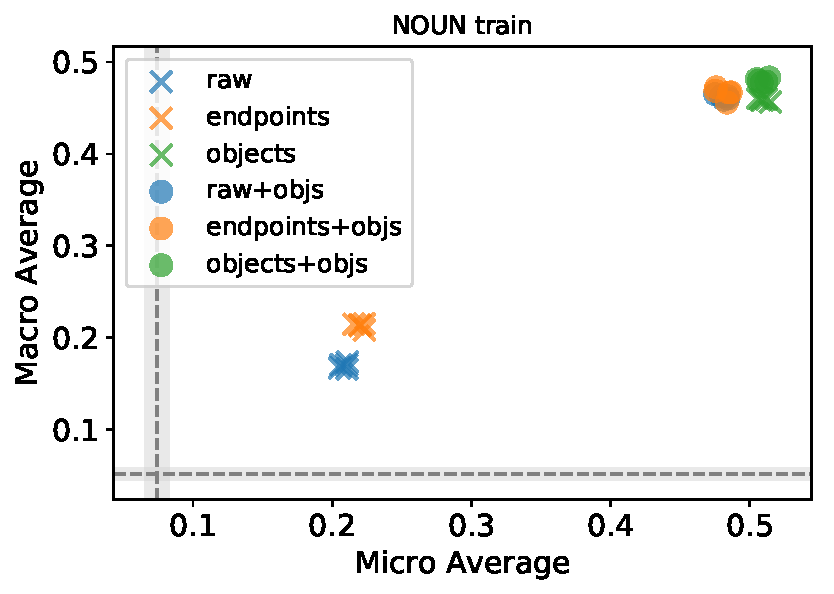
\includegraphics[width=0.5\linewidth]{figures/macromicro_scatter_NOUN_train_dr=False}}%
\subfigure{%
\label{fig:first}%
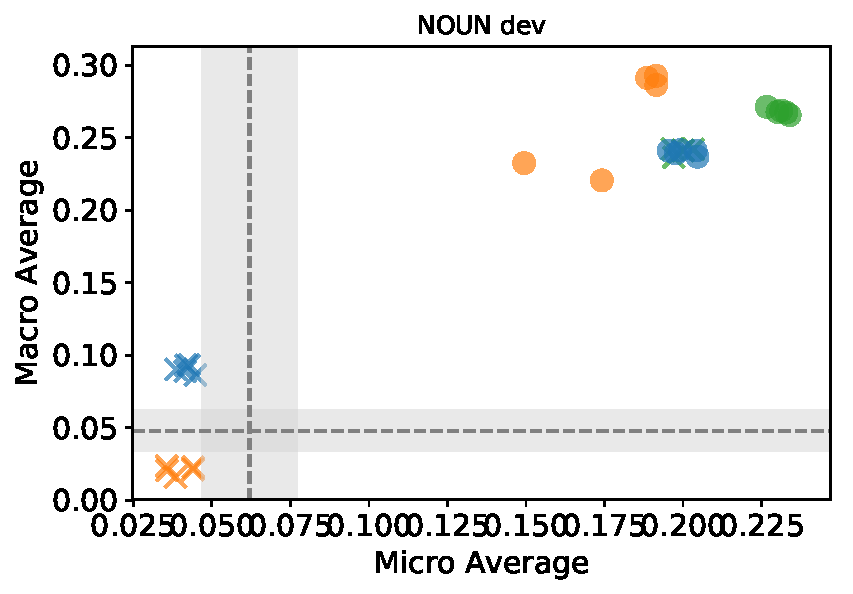
\includegraphics[width=0.5\linewidth]{figures/macromicro_scatter_NOUN_dev_dr=False}}
\subfigure{%
\label{fig:first}%
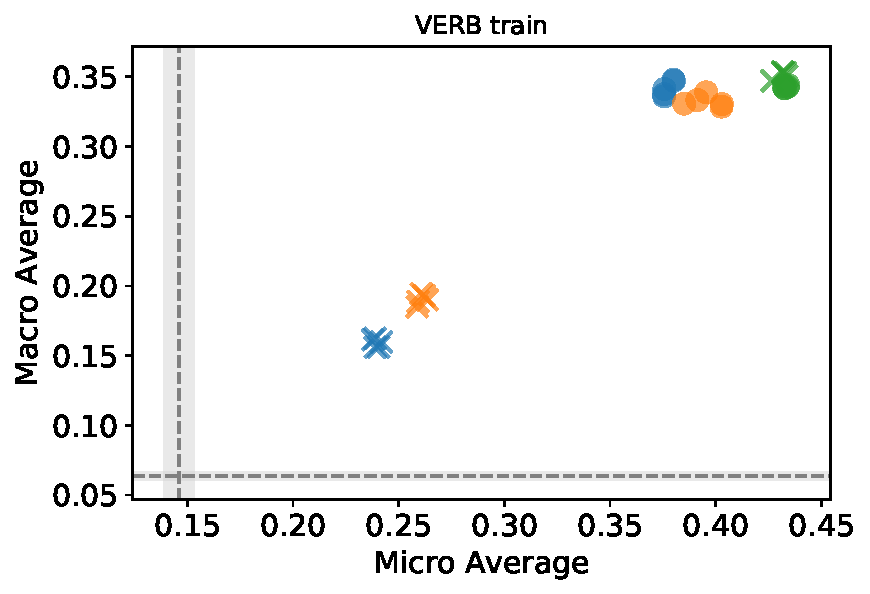
\includegraphics[width=0.5\linewidth]{figures/macromicro_scatter_VERB_train_dr=False}}%
\subfigure{%
\label{fig:first}%
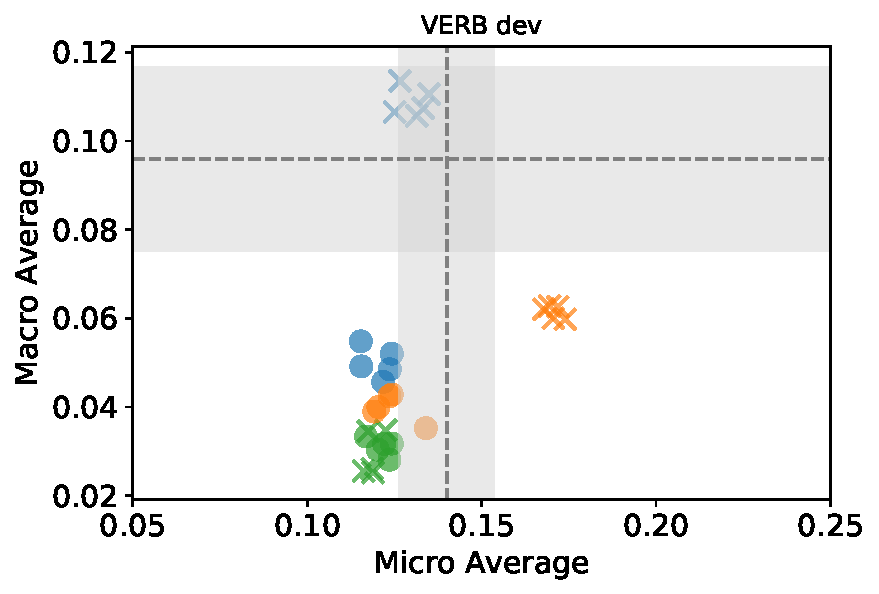
\includegraphics[width=0.5\linewidth]{figures/macromicro_scatter_VERB_dev_dr=False}}%
\caption{Noun representations which include object information perform (unsurprisingly) well. No verb representations perform above chance on dev.}
\end{figure*}

\begin{figure*}[ht!]
\centering
\subfigure{%
\label{fig:first}%
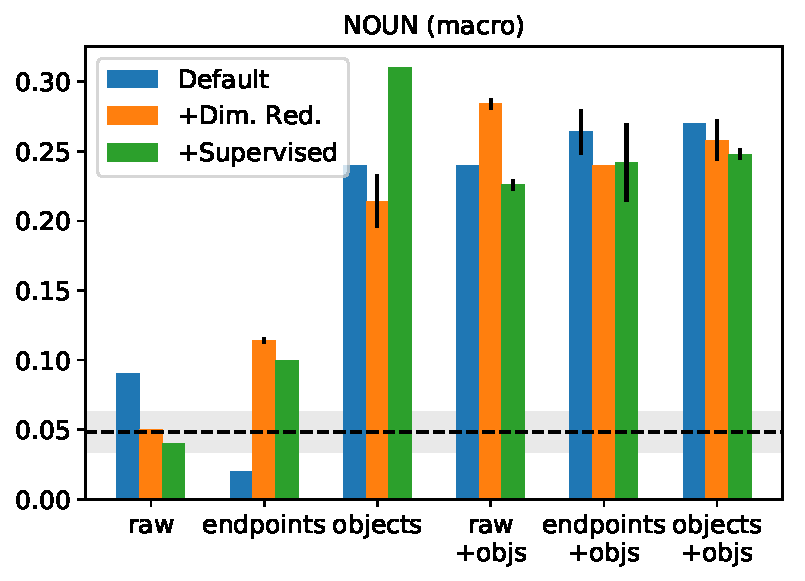
\includegraphics[width=0.5\linewidth]{figures/dr_bars_NOUN__macro_dev}}%
\subfigure{%
\label{fig:first}%
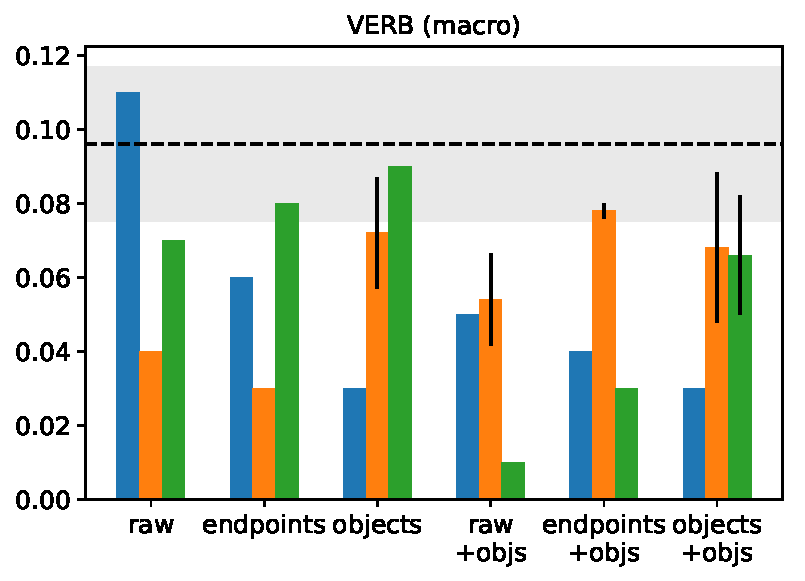
\includegraphics[width=0.5\linewidth]{figures/dr_bars_VERB__macro_dev}}
\subfigure{%
\label{fig:first}%
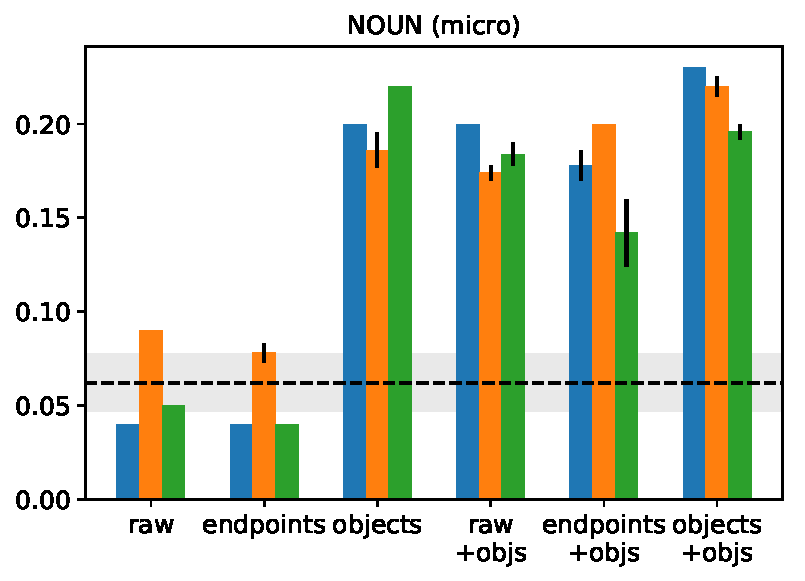
\includegraphics[width=0.5\linewidth]{figures/dr_bars_NOUN__micro_dev}}%
\subfigure{%
\label{fig:first}%
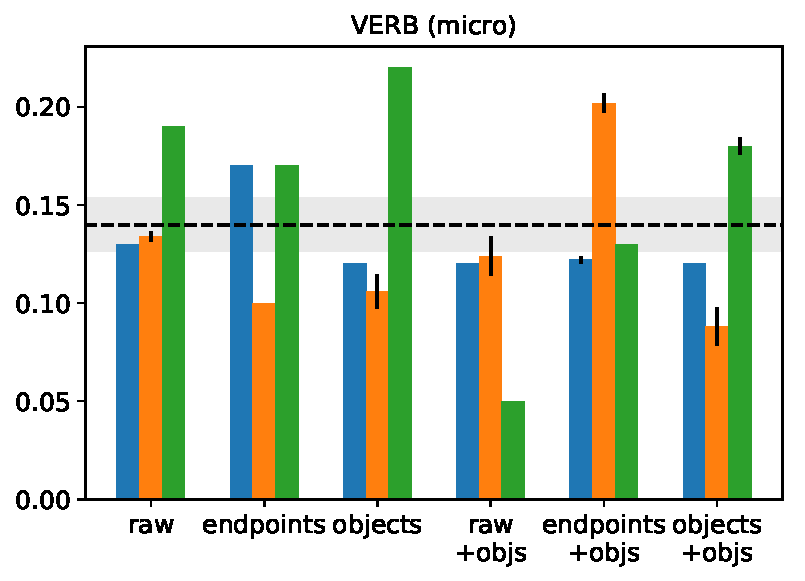
\includegraphics[width=0.5\linewidth]{figures/dr_bars_VERB__micro_dev}}%
\caption{TODO}
\end{figure*}


\begin{figure*}[ht!]
\centering
\subfigure[Clusters, Unsupervised]{%
\label{fig:first}%
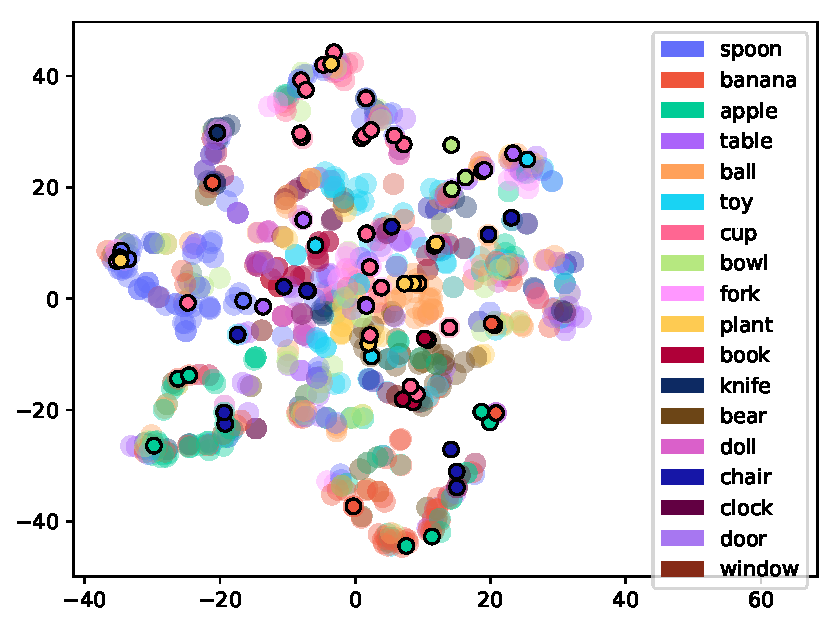
\includegraphics[width=0.5\linewidth]{figures/cluster_viz_NOUN_unsupervised}}%
\subfigure[Confusion Matrix, Unsupervised]{%
\label{fig:first}%
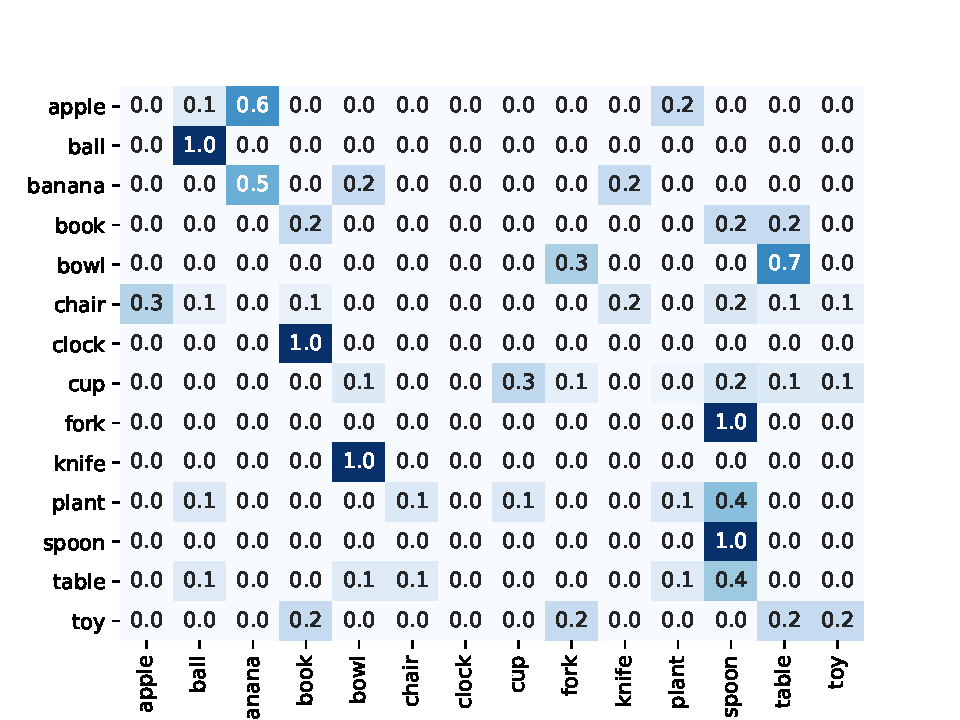
\includegraphics[width=0.5\linewidth]{figures/cm_NOUN_unsupervised}}
\subfigure[Clusters, Supervised]{%
\label{fig:first}%
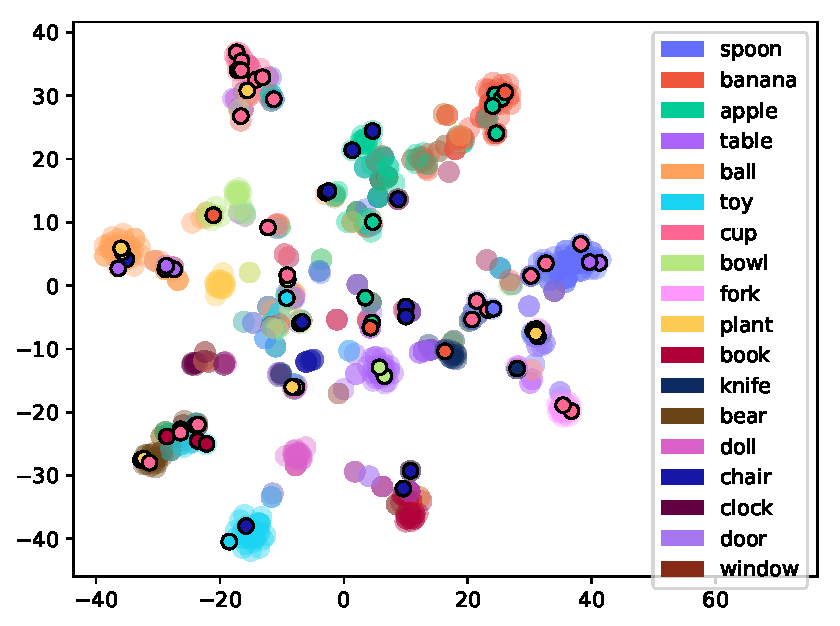
\includegraphics[width=0.5\linewidth]{figures/cluster_viz_NOUN_supervised}}%
\subfigure[Confusion Matrix, Supervised]{%
\label{fig:first}%
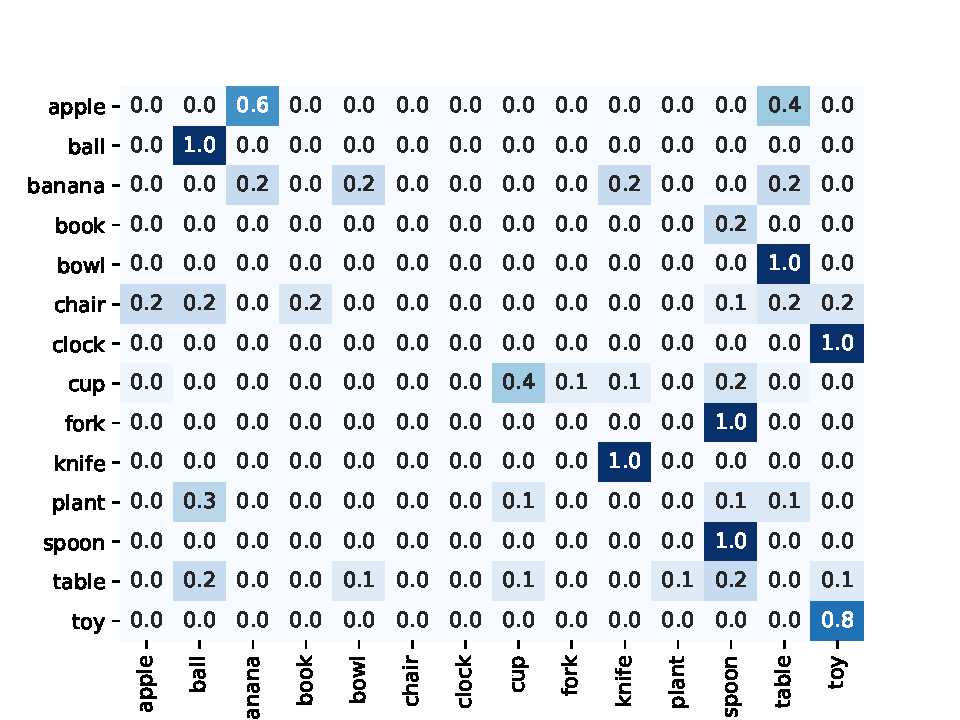
\includegraphics[width=0.5\linewidth]{figures/cm_NOUN_supervised}}%
\caption{Side by side of noun clustering, with vs. without supervision. These are results for the object-based state symbols, but no additional objects added as features. I.e. the blue and green bars under the group labeled ``objects'' in Figure \ref{}.}
\end{figure*}

\begin{figure*}[ht!]
\centering
\subfigure[Clusters, Raw]{%
\label{fig:first}%
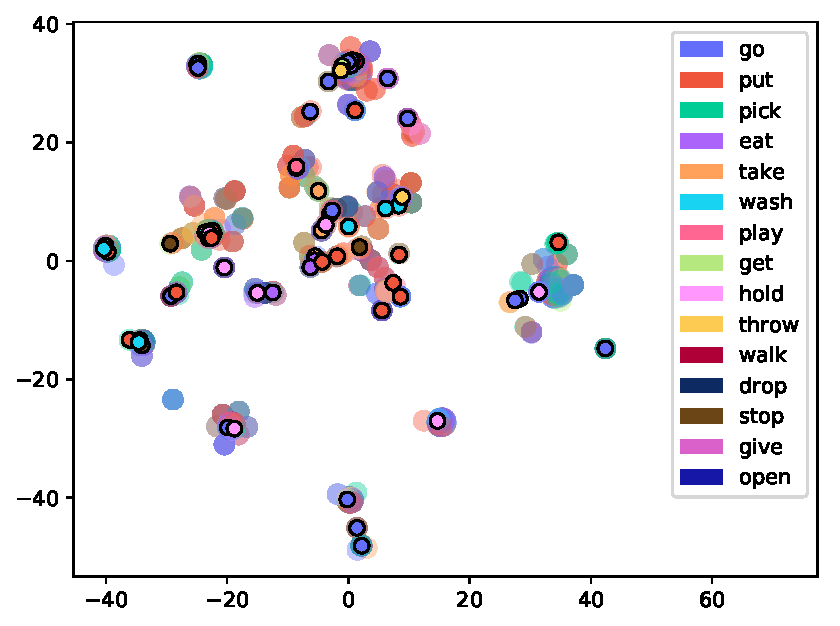
\includegraphics[width=0.5\linewidth]{figures/cluster_viz_VERB_raw}}%
\subfigure[Confusion Matrix, Raw]{%
\label{fig:first}%
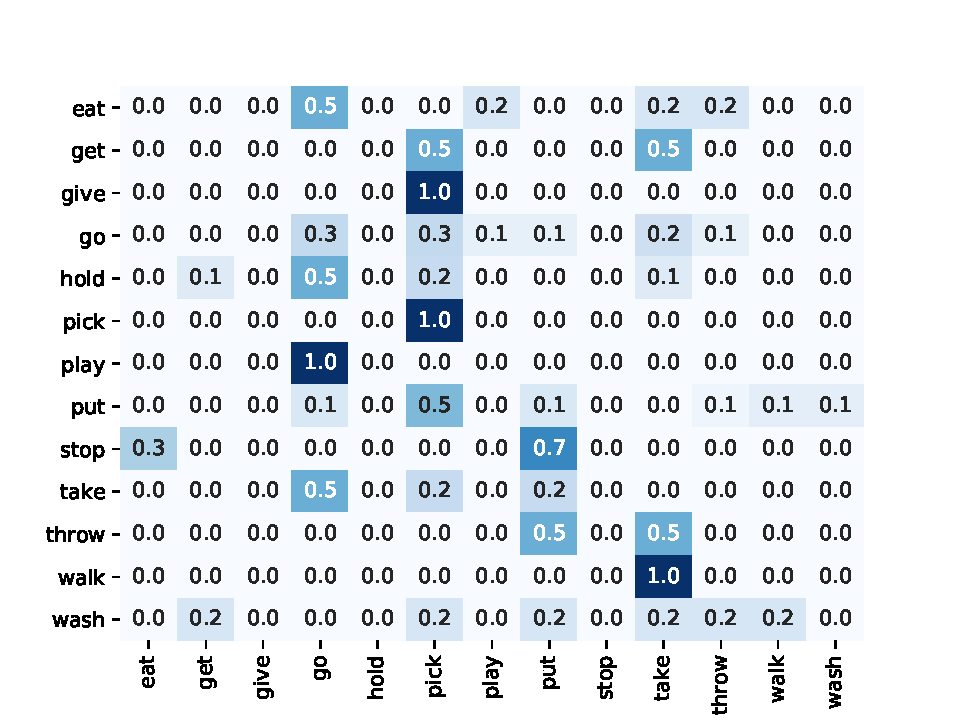
\includegraphics[width=0.5\linewidth]{figures/cm_VERB_raw}}
\subfigure[Clusters, Objects]{%
\label{fig:first}%
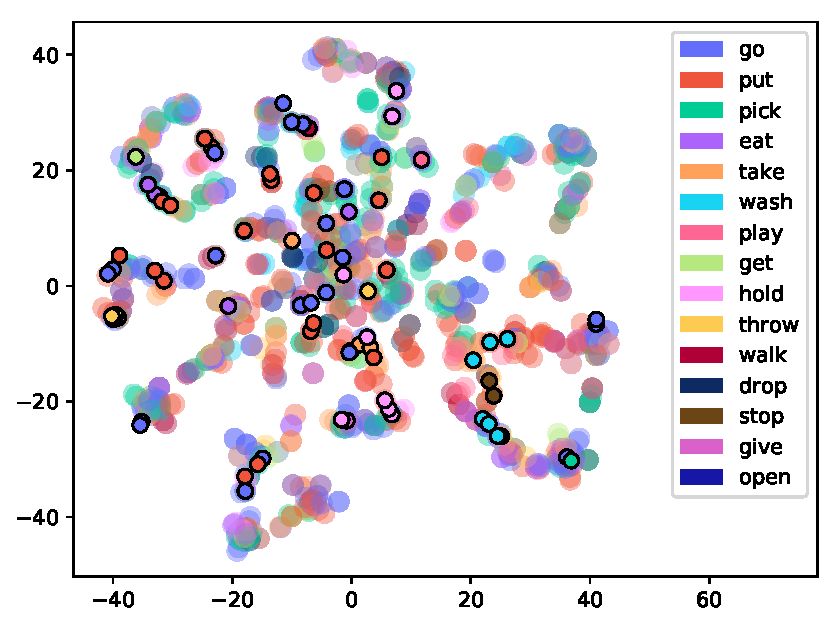
\includegraphics[width=0.5\linewidth]{figures/cluster_viz_VERB_objects}}%
\subfigure[Confusion Matrix, Objects]{%
\label{fig:first}%
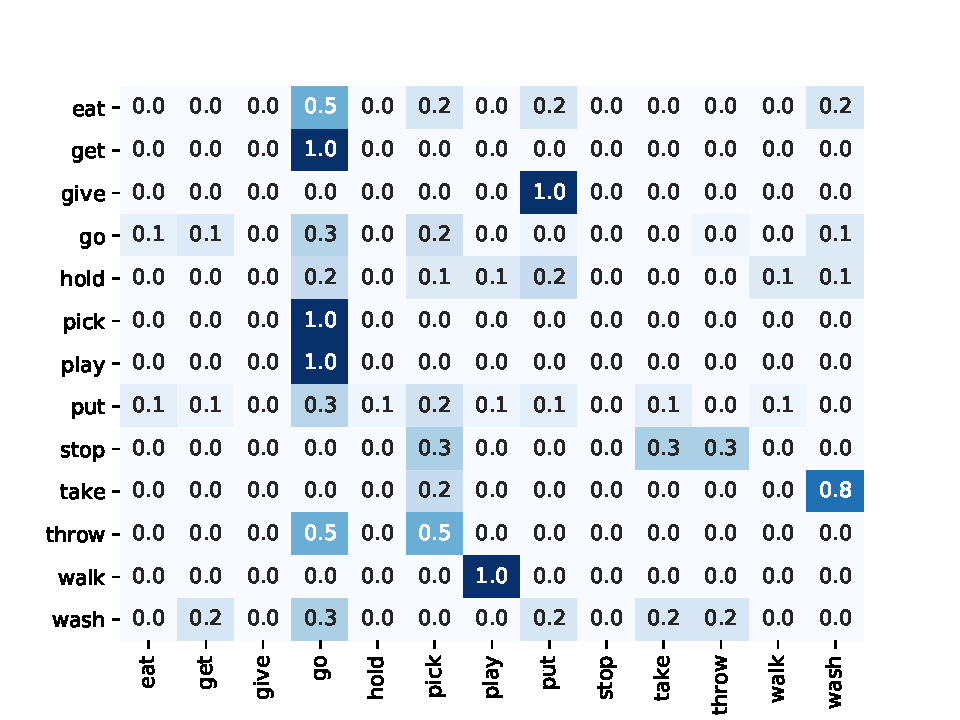
\includegraphics[width=0.5\linewidth]{figures/cm_VERB_objects}}
\subfigure[Clusters, Objects Supervised]{%
\label{fig:first}%
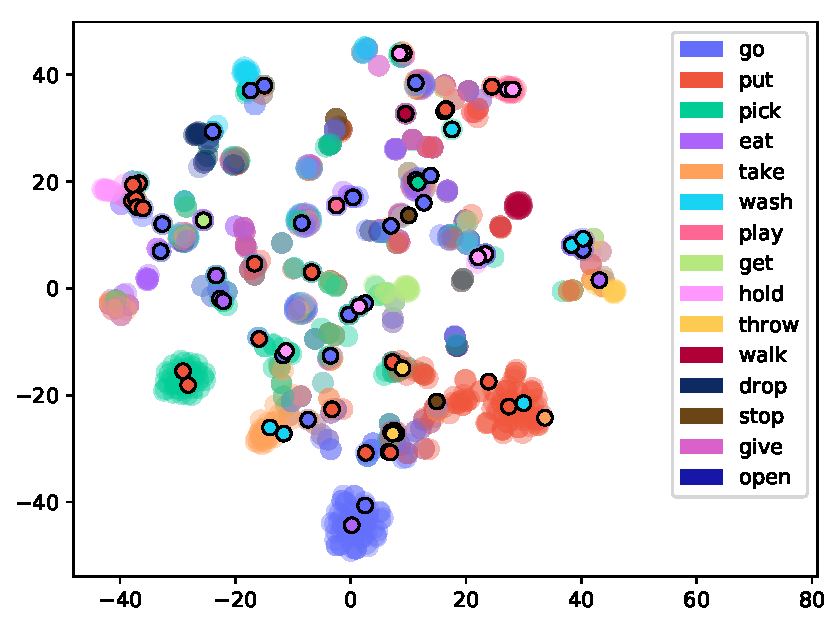
\includegraphics[width=0.5\linewidth]{figures/cluster_viz_VERB_objects_supervised}}%
\subfigure[Confusion Matrix, Objects Supervised]{%
\label{fig:first}%
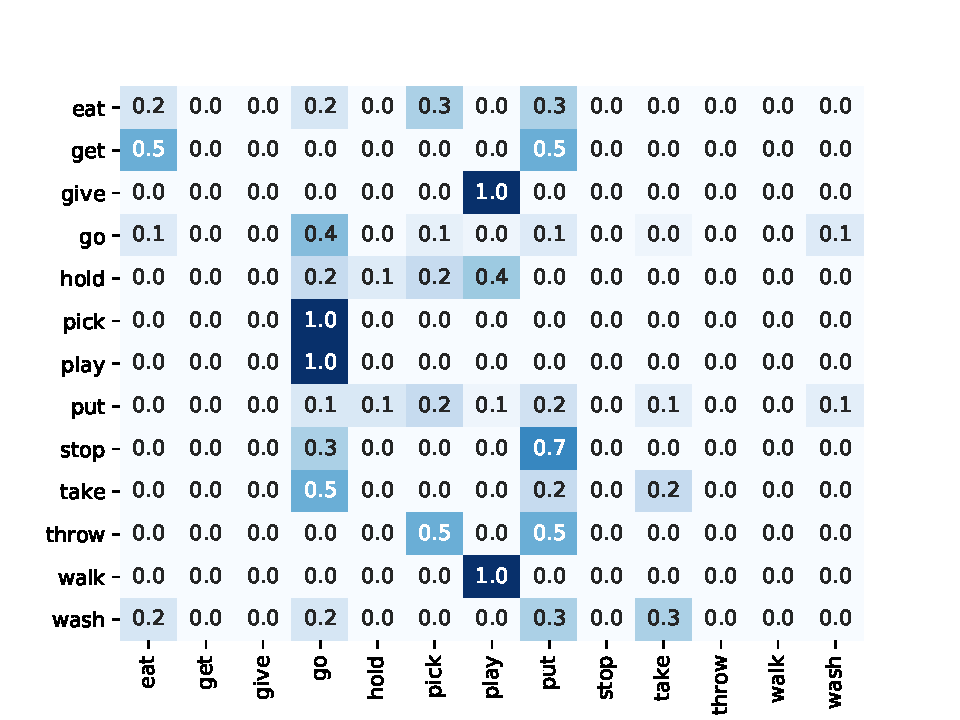
\includegraphics[width=0.5\linewidth]{figures/cm_VERB_objects_supervised}}%
\caption{Side by side of verb clustering. Results are raw, objects, and objects-supervised.}
\end{figure*}


\begin{figure*}[ht!]
\centering
\subfigure[Effect of K]{%
\label{fig:first}%
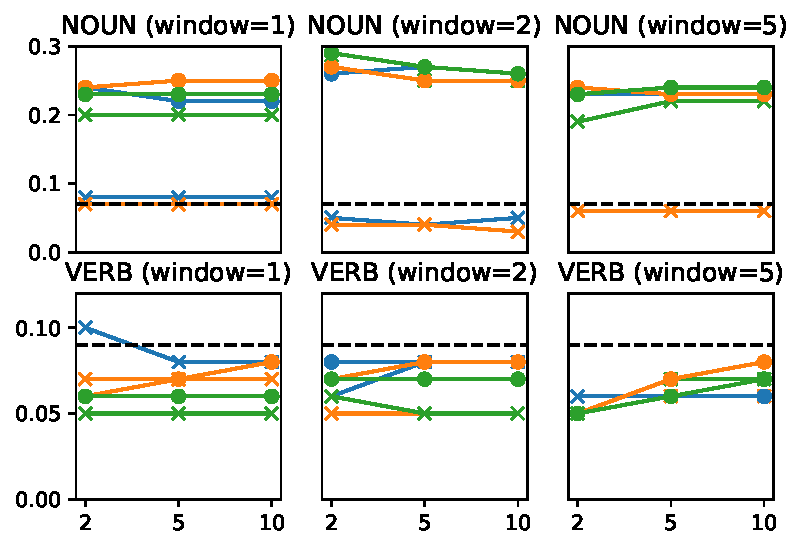
\includegraphics[width=0.5\linewidth]{figures/effect-of-k}}%
\subfigure[Effect of Window]{%
\label{fig:first}%
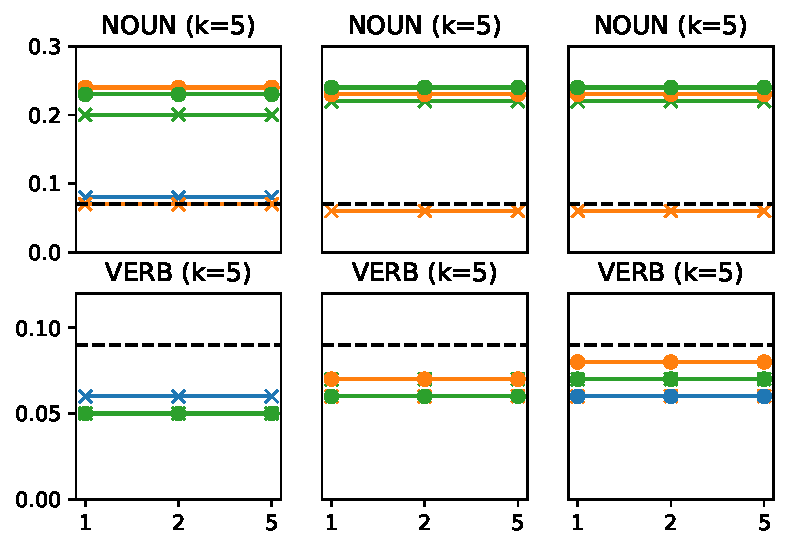
\includegraphics[width=0.5\linewidth]{figures/effect-of-window}}%
\caption{No meaningful effect of window size or ngram length}
\end{figure*}

\subsubsection{Manual Evaluation of Skills}

In this evaluation, for a given selected word-action pair, the word is presented with 10 randomly sampled video segments representing the corresponding action. Words from our target vocab are used, as well as words from max-pmi action-word pairs.

For each sampled video segment, I annotate whether the word matches the video. The answer choices are yes, no, or unsure. Results from the target vocab are:

\begin{figure*}
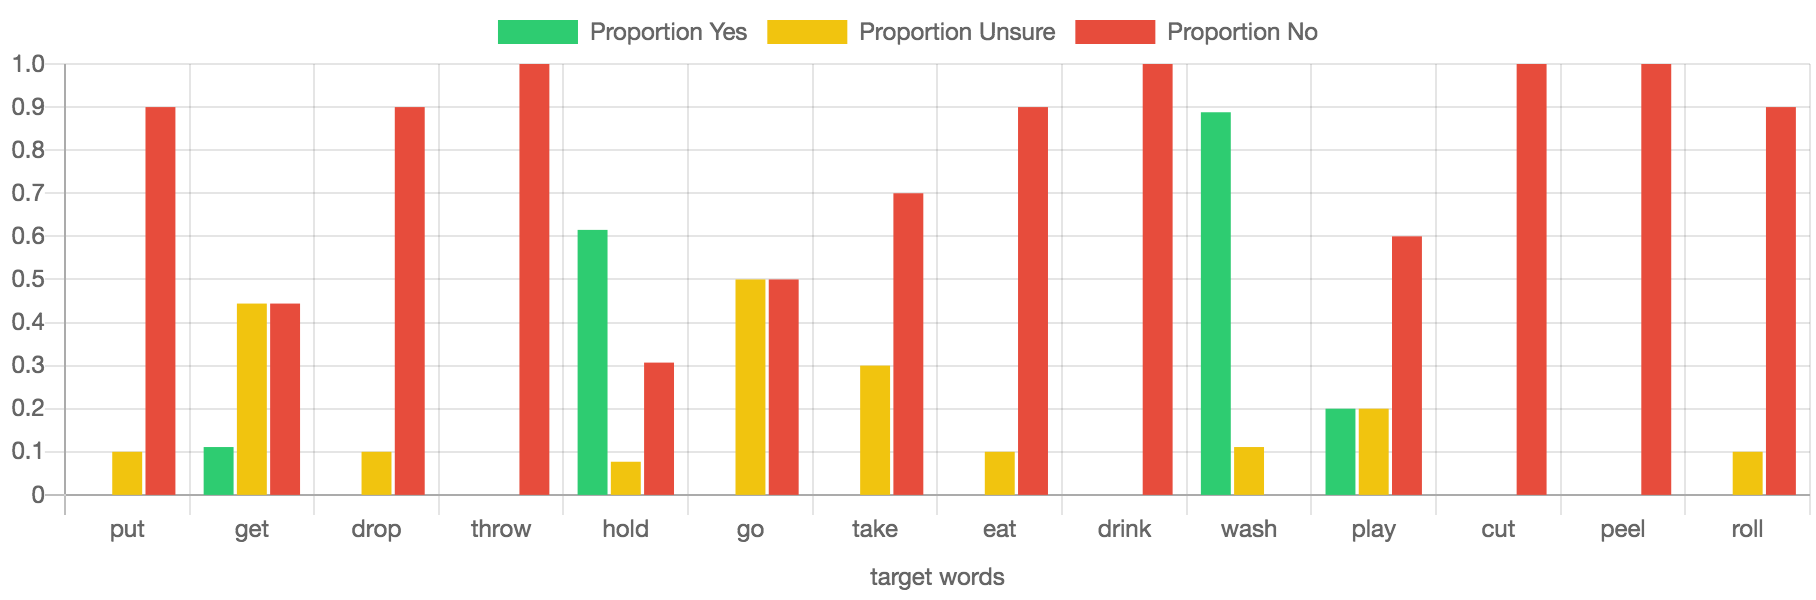
\includegraphics[width=\linewidth]{figures/human_eval}
\end{figure*}

\section{Video Retrieval} 
\label{sec:ir}

To aid in bottom-up language and scene understanding, we have been working towards scene memorization (retrieval) and generalization (captioning) functionality. Concretely, there have been two major lines of work to support better cross-modal retrieval performance: 

1) To avoid pitfalls in negative sample selection/generation processes, we are training our rankers on raw list-wise preference data that allows for significant improvements in ranking effectiveness and drastically reduced model training time for arbitrary existing retrieval models. See Figure 1 for evaluation results on a standard retrieval collection. This work is currently under review at ACM SIGIR.

2) To improve generality and coverage of given scenes and narrations, we have been working on transformer-based query expansion schemes in the latent representation space. Expansion candidates are obtained via a separate transformer model trained on scene-internal frame re-ordering and are then re-ranked based on semantic similarity to the original example. After promising initial results at the TREC 2019 benchmark, we are now working on translating this performance to more resource-constrained settings.

Moving forward, we are combining the above techniques to design a joint textual-visual embedding space via which we will facilitate retrieval and captioning of scenes and that will eventually feed back into our language understanding efforts. 

\begin{figure*}[ht!]
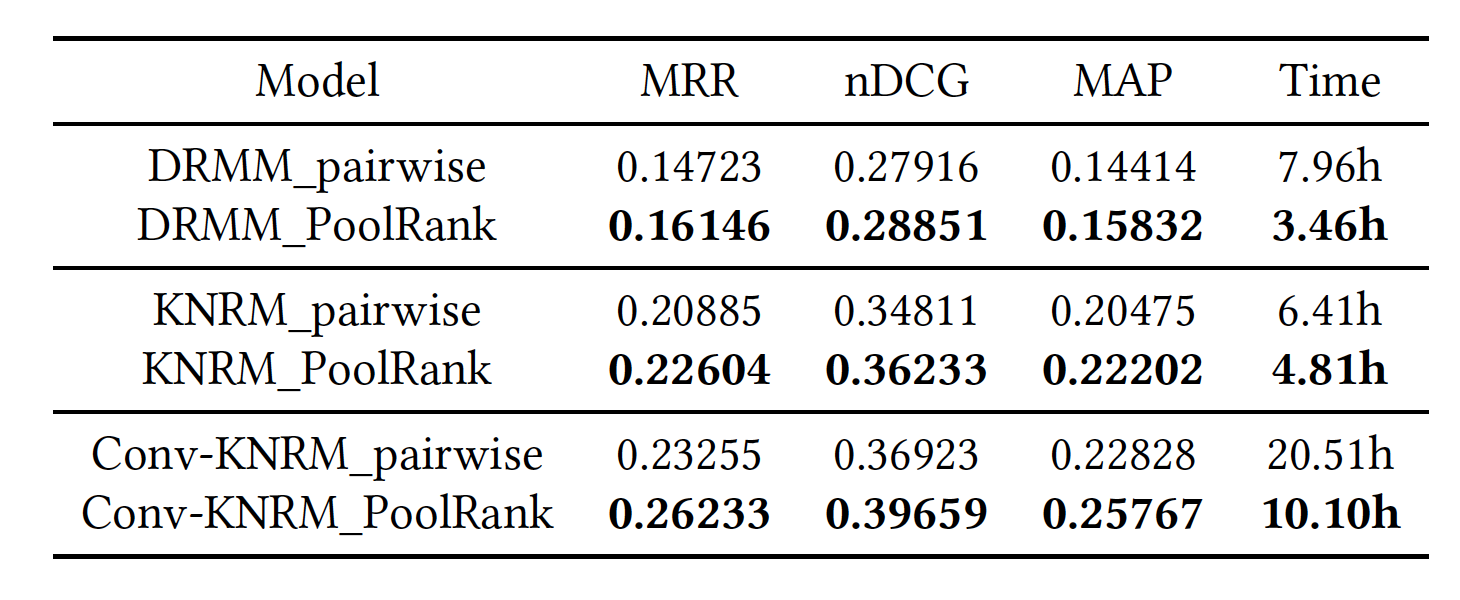
\includegraphics[width=\linewidth]{figures/ir-table}
\caption{TODO}
\end{figure*}


\section{Human Simulation for Function Word Acquisition} 
\label{sec:hsr}

On studies with children: Just before the COVID-19 pandemic hit, we completed data collection on two projects looking at children's learning of logical words. One project has tested over 200 children between the ages of 3 and 7 years old on their understanding of novel quantifier words (how do children learn words like "all" and "some", and how might they extend this procedure to new words in the same syntactic position and sentence frames, like "give me dax of the toys". The other has tested 60 children between ages 3-5 on their understanding of Negative Polarity Items (words like "any" and "much", which are only grammatical in the context of negative sentences). These projects involve two undergraduate thesis students, who are currently processing the data, analyzing it, and writing up the results for their undergraduate theses.

On studies with adults: We have identified a video corpus of parents' speech to a child (SayCAM corpus, entries for Asa) that we can use to develop materials for online studies. This corpus has longitudinal data: approximately 1-2 hours of video recorded from the child's perspective every week between the child's ages of 6 to 23 months (although months 18-23 have not yet been made available). It also has the filmed parents' permissions for others to view video clips from the corpus, including permission to show videos to participants on Amazon Mechanical Turk or other online platforms, which will form the participant pool for the studies we do with these materials. We have machine-transcribed the entire available corpus to identify instances of specific words being used, paired with timestamp information that helps find the corresponding points in the videos. After that, each instance of the words "no" and "not" (over 3,500) has been manually coded by two research assistants to identify the function of negation that the speaker meant to express (e.g. rejection of an offer being made, denial of the truth of another statement, etc.) Currently, we are in the process of identifying videos in which the negation words are spoken by the parents (rather than the kids), which are spoken to the children (rather than to other adults or in another room), and which both coders have agreed on the function of negation being used. We have also completed an extensive preregistration of this project's materials and hypotheses, which lays out this complex data processing pipeline in detail for compliance within our own research team, and transparency and replication by others in the future. The next steps are to trim and process these video clips to create multiple versions for the different experimental conditions we plan to compare to each other. These activities have recently been delayed by research assistants' limited availability as they have had to move off-campus due to the COVID-19 pandemic. However, online data collection should not be impeded by the pandemic once stimulus creation is complete.
 
\bibliographystyle{abbrv}
\bibliography{refs} 
 
\end{document}

